\section{Hilfsstromversorgung}
Mit der Hilfsstromversorgung sind sämtliche Komponenten gemeint, die nicht direkt zum Antrieb gehören. Diese Bauteile laufen mit einer Spannung von $12$ VDC, welche von einem Spannungswandler aus einer Batterie gewonnen wird. Dabei wird eine leichte Asymmetrie der Batterien toleriert, da diese beim Parallelschalten durch den Stufenschalter ausgeglichen werden (durch die stärkere Belastung der volleren Batterie).

\subsection{Steuerplatine}
Um die Kommunikation zu und von den beiden Steuerplatinen zu implementieren, wurde eine sogenannte Steuerplatine erstellt. Diese regelt sämtliche Funktionen, welche mit dem BMS zu tun haben. Das Schema dieser Steuerplatine ist im Anhang unter \ref{Anh_Steuerplatine} zu finden. Dort sind einzelne Bereiche eingefärbt, auf welche im Folgenden eingegangen werden soll.

\paragraph{Gelb: Anschlüsse}
Die gelb hinterlegten Komponenten bilden die Verbindung zu den weiteren Komponenten. Mit Ausnahme der $12$ V-Zuleitung wurden sämtliche Verbindungen als Schraubklemmen ausgeführt. Lediglich letztere wurde aufgrund des grossen Stromes und der benachbarten Montage direkt aufgelötet. Die einzelnen Verbindungen erfüllen folgende Aufgaben: \begin{itemize}
	\item \textbf{BMS1 / BMS2}: Verbindung zum ersten und zweiten Batteriemanagementsystem
	\item \textbf{12Fahren}: Die $12$ V-Spannungsversorgung, wenn das Fahrzeug eingeschaltet ist
	\item \textbf{Voltmeter}: Verbindung zur Batteriestandanzeige
	\item \textbf{Hauptschalter}: Verbindung zu den Spulenkontakten des Hauptschalters
	\item \textbf{230}: Verbindung zum $230$ VAC-Eingang, sowie den beiden Ladegeräten
	\item \textbf{Luefter1 / Luefter2}: Verbindung zu den beiden Batteriekühlern
\end{itemize}

\paragraph{Rot: Spannungsversorgung}
Die Spannungsversorgung regelt, wie der Name bereits andeutet, die Versorgung der Steuerung mit Spannung. Dabei sind die beiden Fälle für das eingeschaltete Fahrzeug (Zustand "Fahren") sowie für den Zustand "Laden" zu unterscheiden.

Beim Zustand \textbf{Fahren} wird die gesamte Steuerung über den im Fahrzeug eingebauten DC-DC-Wandler versorgt, der ausserdem die Beleuchtung mit Spannung beliefert. In diesem Zustand sind sämtliche Funktionen verfügbar. Ausserdem werden die $24$ V des BMS durch die Diode $D_1$ und den Spannungswander $U_3$ bereitgestellt. Die Dioden sorgen dabei für die Trennung der beiden Spannungswandler.

Beim \textbf{Laden} ist es wichtig, dass das Fahrzeug nicht eingeschaltet werden kann. Damit wird verhindert, dass versehentlich mit dem noch eingesteckten Fahrzeug losgefahren wird. Dies wird dadurch sichergestellt, dass das Relais $U_4$ beim Anschluss von $230$ VAC automatisch die Spannungszufuhr für die Steuerung unterbricht. Da jedoch auch beim Laden das BMS eingeschaltet sein soll, wird dieses über einen Spannungswandler vom $230$ VAC-Netz versorgt.

\paragraph{Grau: Passive Signale}
Die beiden passiven Signale umfassen die Information, dass das System eingeschaltet ist beziehungsweise am $230$ VAC-Netz angeschlossen ist. Dies sind logische 0-(entspricht $<1$ V) und 1-(entspricht $>4$ V) Signale. Da bei beiden Zuständen jeweils eine eigene $12$ V Versorgungsspannung benötigt wird, können die benötigten Signale einfach mittels passivem Spannungsteiler aus diesen Versorgungsspannungen hergestellt werden. Die Signale sind ausserdem für beide Batteriemanagementsysteme gleich.

\paragraph{Grün: Relais für die Ladegeräte}
Das Batteriemanagementsystem steuert die Ladegeräte lediglich dadurch, dass sie ein- und ausgeschaltet werden. Diese Schaltvorgänge werden über die beiden Relais $U_1$ und $U_5$ durchgeführt. Dabei ist es wichtig, dass beide Ladegeräte unabhängig ein- und ausgeschaltet werden können. Entsprechend sind auch einzelne Relais vorhanden.

\paragraph{Violett: Treiberstufe}
Die Signale des BMS sind zu schwach, um damit direkt ein Relais oder die Lüfter anzusteuern. Aus diesem Grund werden diese Signale mit Hilfe von MOSFETs verstärkt. Da für das Durchschalten der MOSFETs am Gate eine höhere Spannung anliegen muss als am Sourceanschluss, wurde letzterer mit Masse verbunden und das zu schaltende Bauelement am Drainanschluss angeschlossen. Am Beispiel der ersten Treiberstufe mit $Q_3$ soll dies erklärt werden:

Vom BMS her wird ein Signal zur Verfügung gestellt, welches das erste Ladegerät ein- beziehungsweise ausschaltet. Dieses Signal wird an den Gateanschluss des Transistors angeschlossen. Damit sich dieser nicht zu schnell auflädt, ist der Widerstand $R_7$ in Serie dazu geschaltet. Ein kleinerer Widerstand würde zwar eine höhere Schaltgeschwindigkeit erlauben, dies ist jedoch hier nicht nötig. Der Widerstand $R_8$ sorgt dafür, dass der Gateanschluss in jedem Fall ein Bezugspotential hat. Bei fehlendem Eingangssignal wird das Gate also hochohmig geerdet.

\color{blue}
Bei den Tests hat sich gezeigt, dass die gewählte Schaltung nicht funktioniert. Ursprünglich wurde vermutet, dass das Invertieren des Signals im BMS ebenfalls den Signalpegel invertiert, was sich als falsch herausstellte, da nur der logische Wert invertiert wurde. Aus diesem Grund wurde eine vorgeschaltete Inverterstufe realisiert, welche die jeweils drei Signale pro BMS vorgängig invertiert, um sie so der Schaltung nutzbar zu machen. Diese Schaltung wurde mit einem Schmitt-Trigger realisiert, wobei auch hier die Schaltgeschwindigkeit keine wichtige Rolle spielt. Abbildung \ref{fig:Inverter} zeigt das Schema eines Inverters, für den Aufbau wurde ein sechsfach-Baustein verwendet:

\begin{figure}[h]
	\centering
		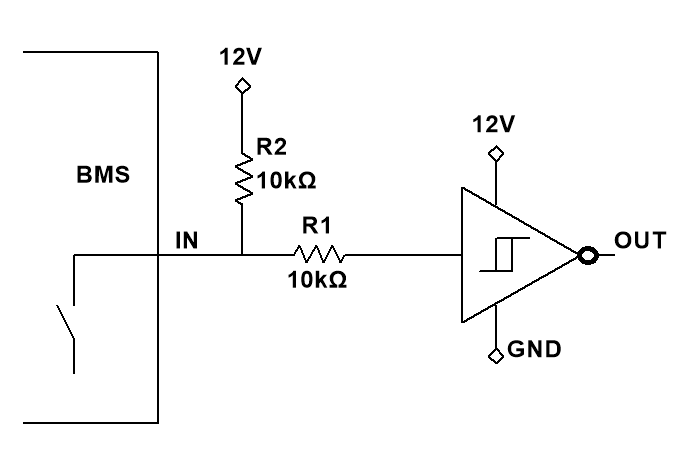
\includegraphics[width=.60\textwidth]{images/Inverter.png}
	\caption{\textcolor{blue}{Die Inverterschaltung, welche sechs mal verwendet wurde}}
	\label{fig:Inverter}
\end{figure}
\color{black}

\paragraph{Blau: Ladezustand}
Da beide Batterien von unabhängigen Batteriemanagementsystemen überwacht werden, können sie auch einen unterschiedlichen Ladezustand aufweisen. Es ist deswegen zweckmässig, den jeweils tieferen Ladestand anzeigen zu lassen, um damit den schlechtesten Fall abzudecken. Diese Signale werden vom BMS in Form eines $5$ kHz PWM-Signales zur Verfügung gestellt. Die Idee des Herstellers ist, dass dieses Signal direkt auf ein analoges Messgerät eingespeist wird, dessen Massenträgheit das Signal glättet. Da beim Detroit lediglich ein Anzeigegerät zur Verfügung steht, müssen diese Signale bereits vorzeitig verglichen werden.

Aus diesem Grund werden die beiden Signale zuerst durch ein eingangsseitiges Tiefpassfilter geglättet. Die Operationsverstärkerstufe $U_{7A}$ vergleicht anschliessend die beiden Signale und gibt ein Signal 0 oder 1 aus, je nachdem, nach welchem Tiefpass eine höhere Spannung anliegt. Um unnötige Schaltvorgänge bei beinahe gleichen Signalen zu verhindern, ist mit Hilfe der beiden Widerstände $R_{19}$ und $R_{20}$ eine Hysterese eingebaut.

Der Transistor $Q_1$ kann mit dem Signal von $U_{7A}$ direkt angesteuert werden. Da jedoch im umgekehrten Fall ebenfalls ein MOSFET verwendet werden soll, muss dieses Signal invertiert werden. Zu diesem Zweck vergleicht der Operationsverstärker $U_{7B}$ dieses Signal mit der halben Versorgungsspannung, wobei das Signal 1 deutlich über dieser liegt, das Signal 0 deutlich darunter. Dieses invertierte Signal wird an das Gate des Transistors $Q_2$ angelegt.

Es steht nun eine Spannung zur Verfügung, welche dem jeweils tieferen der beiden geglätteten PWM-Signalen entspricht. Da das verwendete Voltmeter jedoch verhältnismässig niederohmig ist, wird mit dem Operationsverstärker $U_{7C}$ und dem MOSFET $Q_9$ eine Spannungsfolgerschaltung gebildet. Der Operationsverstärker vergleicht dabei sein Eingangssignal mit der Spannung, welche am Ausgang des Spannungsfolgers anliegt.

Auch bei dieser Schaltung müssen die MOSFETs nur vergleichsweise langsam schalten. Aus diesem Grund wurde für deren Anschluss die selbe Schaltung wie bei den Treiberstufen gewählt. Lediglich beim Spannungsfolger wurde davon abgewichen. Da der Spannungsteiler der beiden Widerstände $R_{27}$ und $R_{28}$ die Spannung nicht verfälschen soll, ist der Gateanschluss über das Voltmeter mit Masse verbunden. Die Idee dahinter ist, dass bei ausgeschaltetem Eingangssignal der Innenwiderstand des Messgerätes im Vergleich zu $R_{28}$ klein ist, also sowieso nicht ins Gewicht fällt. Bei Funktion der Schaltung existiert der Spannungsteiler aber praktisch nicht, da über dem Widerstand lediglich eine sehr kleine Spannung anliegt.